\chapter{Antecedents of Modern Urban Rent Theory: Rent and Production} \label{chapter-rent}

\epigraph{Of the concrete forms of income that have usually been classed as surplus, the rent of land was the earliest to be defined; and so prominent a position has been given to it that the terms `rent' and `surplus' have come to be used interchangeably.}{Alvin Saunders Johnson, 1902 \cite{johnsonRentModernEconomic1902}}
\epigraph{The law of rent has become an obstacle to scientific progress: it has retarded the attainment of a true theory of distribution \dots % Yet it is itself capable of affording such a theory. 
The principle that has been made to govern the income derived from land actually governs those derived from capital and from labor. 
}{John Bates Clark, 1891 \cite{clarkDistributionDeterminedLaw1891}}

% HOW ARE PEOPLE MISUNDERSTANDING RENT - E.G. FROM THE CASE
% IT WAS CALLED POLITICAL ECONOMY
% WHAT BELONGS IN INTRO? RICARDO AND HIS HISTORICAL CONTEXT SEEMS TO GO INTO MORE DEPTH. NEED TO FOCUS OF INTRODUCING RENT, ITS DEFINITION AND IT'S RELATIONSHIP TO LOCATIONAL VALUE AND DISTRIBUTION OF SURPLUS AND GENERALLY RELATIONSHIP. 
% FINANCIALIZATION OF HOUSING MARKET IS IN SPACE - LOCATIONAL..
% STREAM OF BENEFITS \dots DRAWING OUT THE RELATIONSHIP BETWEEN DIFFERENT TYPES OF VALUE OF LAND AND HOW LOCATIONAL VALUE MATTERS \dots IS IN RICARDO AS EXTENSIVE MARGIN - 
% ADD 2 MEANINGS OF MARGIN WHICH RELATE TO THE TWO FORMS OF VALUE PROVIDED BY LAND.
% To build a model of financialization, we need to bring in a concept of rent, that was central in classical economics, but has not been as important in formal neoclassical modeling.
% which is described in the next chapter and to which this thesis contributes. 
% We trace the development of theories of income distribution through the classical and neoclassical periods to provide context to our contribution to the development of a modern urban rent theory.  
% We correct that omission because they are
% Along the way, we also explain how the competing approach to distribution, has perhaps unintentionally left most
%For economists, the word normally means the \gls{surplus} income produced by a scarce factor of production that is created by nature. 
%NEW \Gls{rent}, in economic theory is therefore, not the amount a tenant pays a landlord every month. It  nor is it simply a payment for access to the services provided by the land or another facility.  The economist's notion thus overlaps with, but is not identical with common usage. 
%It was not created by the landlord, but it appears as income for the landlord. Thus 
 %In a similar way, people pay a higher price for housing near  urban jobs and amenities. Land near the centre of a city provides locational services that are far more valuable than any of its potential agricultural services. Because nature did not make much land close to the city center, these locational services are scarce and command a high price. The extra cost to be close to the center is an \gls{economic rent}. 
% In general, the locational element is ignored but, IT IS ALWAYS OR GENERALLY AT PLAY?. Even in the sports example. 

In an urban economy, land provides benefits in the form of housing, and places for work, storage, commerce and recreation. Location matters in an urban economy because value is generated by bringing people and activities together. The value of a piece of land in a city derives, not from the richness of the soil, but from the richness of the activities it supports and because of the people and activities it provides access to. A range of theorists have struggled to use the classical theory of rent developed by classical eocnomists in the 19$^{th}$ Century to explain the problems and crises of the modern city, its form, and even its future \cite{hailaTheoryLandRent1990, jagerUrbanLandRent2003, harveyUrbanProcessCapitalism1978}. This thesis extends that work. 

The economist's notion of rent  overlaps with, but is not identical with common usage. \Gls{rent}, in economic theory is not the amount a tenant pays a landlord every month, nor is it simply a payment for using land or another facility. Originally the term was applied to the payments landowners collected. In classical theory the concept was modified to mean payment for payment for ``the indestructible qualities of the productivity of land'' \cite{Gray1914RentUT}. The economic value of land naturally depends on its location---without  nearby buyers, the product of the land has no market value at all---so while the term rent was used to refer to the payment itself, it was actually referring to locational value of the land. %The value of land is accounted for by the economic concept of rent. 

For modern economists, the word, initially developed to understand the income of landowners, extends to include the \gls{surplus} income produced by any scarce factor of production that is created by nature. %and has locational value. 
People pay a high price for housing near the center of a city because there is a limited amount of land close to the center, and being close to urban jobs and amenities is valuable. The extra payment for being close to the center is an \gls{economic rent}. Land with natural resources like mineral deposits, similarly generates locational rents. 

Economists also talk about scarce talents using the concept of rent.  The natural talents of a sports star like Lionel Messi have great market value and  also generate rents, since people like Messi are very scarce. It may not be obvious to think of Messi as having a locational value, but if his services cannot be delivered to a market willing to pay to watch football, his services as a footballer have little or no economic value.% and he might do better as a housepainter.
\footnote{The market model of football has become almost an inversion of the agricultural market. Stadiums served as the market place where buyers and sellers met, but television now delivers Messi to global market, greatly expanding the rents he can bargain for.} 

In this thesis, we use the concept of rent to model how financialization allows for the capture of a growing share of urban productivity. %This concept of rent provides us with a theory for understanding the distribution of surplus. 
If financialization of the urban housing market is directed to capturing the stream of economic surpluses generated by the city, the theory of rent provides a basis for understanding the allocation of surpluses.

In this chapter, we build a bridge from \gls{classical rent theory} to the modern theory of urban rent, which this thesis works to develop. To do this, we discuss classical and neoclassical theories of rent and production.\footnote{Political  traditionally distinguished (1) absolute  rent, (2) monopoly rent, (3) extensive differential rent and (4) intensive differential rent \cite{jagerUrbanLandRent2003}.  Our exposition deals almost entirely with the third category.  To deal with the others would require minor extensions of our model but relatively large additions to our text.} 
%surplus value. Financialization is about capturing the surplus in an urban economy. 
%we trace the development of antecedents to the work on modern urban rent theory developed in this thesis, beginning with classical tradition of rent, and tracing through the development of the neoclassical tradition, and modern theories of production. 
% The land itself is not better but the location is. %It was not created by the landlord, but it appears as income for the landlord. Thus 
%Property and land have multifaceted benefits that include both what you are using it for and the value of what it is in proximity to.
% Financialization is the capture of surplus. Rent is key to how economists have studied the distribution of the surplus. % It was central in classical economics.
% In order to model what's happening in financialization, we need the concept of rent. https://www.overleaf.com/project/606a6b286ae1c9f203fadab5
% In 1902 Alvin Saunders Johnson \cite{johnsonRentModernEconomic1902} summarized the relationship between rent and surplus in the economic literature as follows: 
% In this thesis, we identify what are essentially \glspl{classical rent} in the urban system and examine their distribution to develop a model of financialization of the urban housing market. 
% We bring in the concept of rent because it is necessary background for our examination of the impact of \gls{financialization} on urban productivity. 
% ***E OR MAYBE OPEN WITH THIS? OR: Economics is the study of ___. It is concerned with production (i.e. ___ and distribution (ie. ___) 
% We use the \gls{Cobb-Douglas} function %, which is used to cross this entire range of literature to illustrate each link and to show how our model is directly connected with this broad collection of linked theories. 
% The \gls{Cobb-Douglas} function is a production function, expressing the output produced, in terms of inputs such as labour and capital.
% Our model connects to the results in this chapter at four points:

% In the following chapters we will discuss the three pieces of theory needed to build a model of financialization, rent, urban spatial models, and growth theories. From there, we will bring these things together into a formal model in Part~\ref{part-model}.
 
 % The question of how wealth is created and distributed has been central to Economics since the discipline emerged. 
 % the land-owning class in the era of the classical economists. % Property ownership has been a central form of wealth throughout history. % one of central forms of  wealth and means of building wealth 
% As the primary source of food, power comes from food, which was the main product. 
%  ADD EXPLANATION % Land ownership traditionally defined the ruling classes. The king would give land as reward. Land is what you would fight wars for. The agricultural surplus , the surplus from the land what allowed civilization and cities to form. Before the industrial revolution, the surplus of  agricultural land. taking ownership used to consolidate wealth and power, in feudalism ownership of land set apart ruling classes/aristocracy, . As pearl buck said "land is everything.." or quote that "the only way to create intergenerational wealth is the rare company that or property ownership.  GIVE EXPLANATION HISTORY OR SUMMARY
% More recently the expansion of European economies across the globe brought huge amounts of land into play and combined with rapidly falling transportation costs, led to a society, especially in the labour-scarce settler societies of North America and Australia with  widely distributed property and  home ownership. 
 % of the early stage of the industrial revolution, % it seemed clear that
 
\section{The classical theory of rent and the distribution}
Cultivated land provides a stream of benefits in the form of agricultural products.
Prior to the industrial revolution, most people in Europe lived on and worked the land, primarily producing food, with ownership concentrated in the hands of a few landowners.  Agricultural production played such a central role in the economy that landownership was the basis of wealth, political power, and social distinction.   

For early economists, all wealth appeared to come from the land. The Physiocrats in particular, a school of \gls{political economy} in 18$^{th}$ century France, emphasized that land is the source of all wealth, that only agricultural labour was genuinely productive.\footnote{They argued, based on the productivity of land, that government policy should not interfere with the operation of natural economic laws. Within this framework, they were the first to frame labour as the source of value. Marx, extending the approach to the industrial economy, generalized the analysis, treating industrial labour as generating a surplus as well, as we discuss in \ref{section-rent-and-industrial-capital}, but excluding other workers.} They argued that tradespeople, professionals, clergy, and aristocrats were nonproductive. 
Rent theory originated in this land-based agricultural society. Landowners controlled access to the means of production and charged for access. 
The income landowners extracted was what economists called \gls{economic rent}, or \gls{land rent}.
Given the importance of land to overall economic productivity, the theory of rent emerged as a primary way of understanding the economy, and therefore the distribution of wealth in this period.
%  to understand the allocation of the surplus product of the land. Rent was the value of the productivity of the land itself after costs. Since costs included the costs of transporting produce to market, land rent was always based on the location of the land. % IS THIS TRUE??? EDIT::
% It was described early as \gls{political economy}.
% What became economics was called \gls{political economy}. MAKE LINKS
% FROM GLOSSARY "Political economy is a branch of social science that studies the relationship  between government and the economy. As a discipline, it dates back the  16$^{th}$ but is usually associated with the political economists of the mid-18$^{th}$ and  early 19$^{th}$  century like Adam Smith who began to explore the economic implications of free markets and industrialization. Departments of political economy persisted well into the mid 20$^{th}$ C before splitting into separate departments of economics politics \cite{helleiner20PoliticalEconomy2018}.
%, and economic analysis naturally focused on the distribution of the rent. % surpluses of the land, rent.
% The physiocratic school of economics was the first to see labour as the sole source of value but, for the physiocrats, in the context of the prevalent European rural society of the time, only agricultural labour created a surplus. 

\subsection{Historical development of classical rent theory}
Alvin Saunders Johnson wrote in 1902 ``[o]f the concrete forms of income that have usually been classed as surplus, the rent of land was the earliest to be defined; and so prominent a position has been given to it that the terms `rent' and `surplus' have come to be used interchangeably'' \cite{johnsonRentModernEconomic1902}. 

David Ricardo provided the canonical presentation of the classical theory of rent \cite{ricardoEssayInfluenceLow1815} in 1815.\footnote{Classical rent theory originated with thinkers such as Richard Cantillon (1680s--1734), Fran\c{c}ois Quesnay (1694--1774), the marquis de Mirabeau (1715--1789), Anne-Robert-Jacques Turgot (1727--1781) and Adam Smith (1723--1790), and received its classic statement in Ricardo (1772--1823). Nearly contemporaneous thinker, Johann Heinrich von Th\"unen (1783--1850) developed a planning model to guide the location of economic activities for an urban-agricultural society. A version of that model was reinvented in urban geography by William Alonso.} 
 Ricardo defines rent in relation to who claims the surplus productivity of the land, %this idea about the productivity of land, and who claims that value, 
saying ``[b]y rent I always mean the remuneration given to the landlord for the use of the original power of the land'' \cite{ricardoEssayInfluenceLow1815}. The key term in that definition is ``the original power of the land.'' In the classical tradition, rent is the surplus produced by labour, using land, that is claimed by landowners by virtue of their ownership of the land. The price of the corn would include payment for working the land and for transporting, storing, and selling the product, but the residual that was rent was a payment for the virtue of the land not the contribution of the landlord.

For Ricardo, \gls{land rent} is thus a kind of \gls{surplus value}, that is, an amount available after the costs of production have been paid, the term rent came to be used interchangeably with this more general concept in much of the classical work on rent and the term rent has been used in a more general sense to other kinds of surplus value, as well as land rents.

In Ricardo's time, economic rent and the rent paid by farmers to use the land were almost interchangeable. Landowners `rented out' land. The level of rent charged might not be exactly the economic rent, but in a labour-surplus economy\footnote{Between 1604 and 1914 over 5,200 enclosure Bills were enacted by Parliament which related to just over a fifth of the total area of England, amounting to some 6.8 million acres. From the 1750s enclosure by parliamentary Act became the norm. In Scotland  between 1750 to 1860 the  Highland Clearances  evicted a significant number of tenants in the Scottish Highlands and Islands, mostly in two phases from 1750 to 1860. Enclosures and clearances created a large pool of essentially minimum wage labour that supported industrialization and drove British migrations to the colonies.} landlords had enormous bargaining power, and charged tenant farmers rents that tended to approximate the value of the \gls{surplus}.\footnote{It is important to remember that there was always a conventional level of rent reflecting the power relations between the classes and anchoring the level of rent extraction that was possible.} 

%, and rent as a price tended to approximate \gls{economic rent}. 
%Ricardo used this concept of rent to build out a theory answered answer the social question `who gets the surplus?' This was an approach to understanding the distribution of wealth.

Ricardo was interested, in particular, in the division of the surplus among the classes of society:  which is to say, to the owners of land, labour, and capital.\begin{quotation}
 ``The produce of the earth---all that is derived from its surface by the united application of labour, machinery, and capital, is divided among three classes of the community; namely, the proprietor of the land, the owner of the stock or capital necessary for its cultivation, and the labourers by whose industry it is cultivated \dots  But in different stages of society, the proportions of the whole produce of the earth which will be allotted to each of these classes, under the names of rent, profit, and wages, will be essentially different''  \cite{ricardoEssayInfluenceLow1815}. CHECK SOURCE.
\end{quotation}
Ricardo's concern with the distribution of the surplus in an agricultural economy reflected the social concerns of his time. Primarily agricultural, the increasing globalization of trade in the early stages of the industrial revolution,\footnote{The Industrial Revolution is usually described as beginning around 1760 and having significantly transformed society by about 1820--1840.} was driving both rising overall wealth and greater poverty for many in the working class.

Understanding rent was essential for policy analysis. The Physiocrats focused on land and on the rents to understand tax policy. Ricardo applied rent theory to explain the effect of tariffs. For Ricardo this theory provided insight into whether Britain should open its doors to corn from the colonies.\footnote{ This was the debate over the Corn Laws (1794-1846), a set of duties on grain imports into Britain to protect British agriculture from outside competition. In Britain, ``corn'' was the generic name for cereal crops. The full title of Ricardo's essay explains his purpose" \textit{An Essay on the Influence of a Low Price of Corn on the Profits of Stock, Showing the Inexpediency of Restrictions on Importation: With Remarks on Mr Malthus' Two Last Publications: `An Inquiry into the Nature and Progress of Rent,' and `The Grounds of an Opinion on the Policy of restricting the Importation of Foreign Corn.'} }

% it was a period increasing overall wealth in Europe, in which in many cases the living condition of the working class declined \cite{GET-industrial-inequality}. The wealth came from the increasing globalization of trade in the early stages of the industrial revolution but seemed to enrich primarily a small class of people in a position to benefit.  
% agriculture and the distribution of the surplus reflected the social concerns of his time.  Europe had primarily agricultural economic system and  %in Northern Europe,  and at a time when the benfits of the social changes seemed to benefit a few. 
% The economic transformations of the period seemed to benefit a small number of people able to claim the gains. 
% He worked during a period of during increasing globalization of trade and the early stages of the industrial revolution,
% In this period, the study of \gls{political economy} was emerging as a subject of study that focused on understanding trade, wealth, and government.\footnote{CHECK/REPHRASE? Prior to this, international relationships centred on studies of the military. As colonization changed the relationship between countries and trade became central, the study of \gls{political economy} became more significant.}


% It's easy enough to see how this concept would evolve into the two different usages of the term rent. Because it is the profit for the land, which is related to payments for the land. At the time, the feudal ownership structures meant that the value of the land was structured differently. Tenants did not pay to occupy the land the way that people and businesses do today. Rather the value of owning land was reflected in the distribution from production. The term later split to reflect both the way land is currently valued (i.e rent payments to occupy) and the surplus value that was how land was valued in the period of clssical econmics with it's feadul structures. Rent became payment to landlord because under feudalism, the surplus went to the landlords. Thenn the term diverged into the two distinct meanings used colloquially and in a technical context by Economists ) 

%The profit now accrues to the landowner, and we call it land rent. For Ricardo, it was obvious that the land-owning class captured the land rent.
% who picks up vegetables at the farm gate, transports them into town, and sells them to a storekeeper. He pays the farmer at one end of the trip and is paid at the other. 

\subsection{Locational value in agricultural markets} \label{section-rent-carter}
Location is at the center of the classical theory of rent. The role of locational value in the theory of \gls{rent} can be illustrated with the story of a carter. The carter transports agricultural products, for instance potatoes, from farms to sell in town. %If the carter has a transportation monopoly---owning the only suitable wagon in the region. 
There is a price for potatoes in town and a lower price at the farm gate. The carter buys potatoes from farmers at the cost of production, transports them to town, and resells them at the higher price in the urban market. What remains of the price gap, after subtracting labour and vehicle costs, is profit. % for the carter. SEPERATE OUT QUESTION OF WHO GETS THE PROFIT.

The cost of transporting the potatoes depends on how close farms are to market.  
%In this story the carter captures all of the land rents by exploiting a transportation monopoly. 
The net return thus declines with distance from town. Beyond a certain distance, the costs of the trip will eat up all profit. That is the farthest distance the carter will travel to purchase potatoes. It marks the \gls{extensive margin} of agriculture. 

\begin{figure}[htb]
\begin{center}
 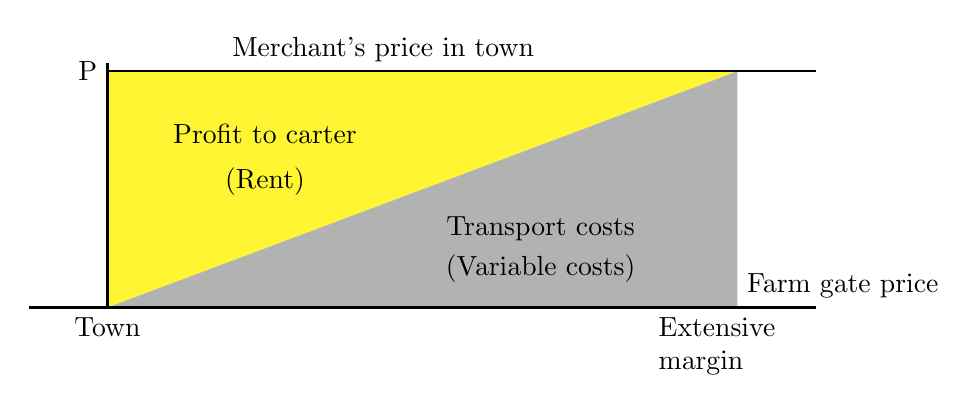
\begin{tikzpicture}[domain=0:2]
%\draw[thick,color=gray,step=.5cm, dashed] (-0.5,-.5) grid (3,3);
%\draw[line width=.01, green ] (0,0) -- (10,0) node[right  ] {Distance};
\node at (1,0) [below] {Town};
\fill[yellow!80]  (1,0) --(9,3)--(1,3) --cycle;
\fill[gray!60] (9,3) --(1,0)--(9,0) --cycle;

\draw[thick ] (1,3)node[left]{P}  -- (10,3);\node at (4.5,3)[above ] {Merchant's price in town} ;
\draw[thick ] (0,0)  -- (10,0); 

%\draw[thick,color=red] (1.5,0) -- (1.5,1) node[below right] {Fixed cost} -- (1.5,1.5) --(10,3.25)node[above left] {total cost};
\draw[thick] (1,0) -- (1,3.1) ;
\node[below,text width=2cm]at (9,0) {Extensive margin};
%\draw[ultra thick, blue,<-> ] (3,1.8) -- (3,2.5)node[left] {annual rent at a} -- (3,3) ; 
\node at (9,0)[above right] {Farm gate price};
\node  at (6.5,1){ Transport costs};
\node  at (6.5,.5){ (Variable costs)};
\node  at (3.,2.2){ Profit to carter};
\node  at (3.,1.6){ (Rent)};
\end{tikzpicture} 
\caption[Ricardo's theory of extensive margin.]{Ricardo's theory of the extensive margin using transportation costs to emphasize the similarity between rent in classical theory and in the Alonso model (developed in  Chapter~\ref{chapter-space}). Transport costs, the darker, gray area, take a share of the profit for vegetables sold in the town}
\label{fig-rent-ricardo}
\end{center}
\end{figure}

 % The extensive margin provides a key insight  into modern urban tent theory. 
% ELABORATE ON WHY EXTENSIVE MARGIN MATTERS. - QQQ FERTILITY VS DISTANCE TO MARKET
% FLIP DESCRIPTION AND CHECK ALIGNS WITH OTHER FIGURES. 

Figure~\ref{fig-rent-ricardo}, shows the total transportation costs as the darker, grey area. The lighter,  yellow triangle is profit for the carter. The carter makes a `profit' on the trip to the farm nearest to town, a smaller profit farther from town, and no profit on any farms beyond this point.\footnote{Note the similarity with Alonso's urban model, illustrated in Figure~\ref{fig-rent-alonso}, in Chapter~\ref{chapter-space}.} 
Together these two triangles represent the  value of the `product of the earth,' but only the upper triangle is a social \gls{surplus}. The lower triangle is the amount of value expended on transportation. The social surplus was termed the `\gls{produit net}' by the Physiocrats. This surplus may go to the landlord, the carter, the merchant or the consumer, depending %on the social relations that prevail. %Land rents may or may not go to the landowner, depending 
on their relative power. 
If the carter has a transportation monopoly---owning the only suitable wagon in the region, the carter may claim the profit. The surplus is called rent if it's captured by the landowner. If if goes to the carter, it's usually called profit. In modern supply and demand analysis it would be recognized as `\gls{producer surplus},' which is the difference between what a producer gets for a good and what they would be willing to accept. 


% LINK The story illustrates that 
% (Carter's expensive dirrectly change the value of the land, dependant on proximity, because they change expenses.
%---reflect the expense incurred depending to proximity to market. 
% Imagine an  town in Ricardo's context, surrounded by potato farms, with people who pulled carts to carry potatoes to sell at a market. 
% Imagine there is one person who owns the only cart in the region that can be used to move potatoes. Now imagine that this monopoly carter notices that 
%, by definition. 
% The surplus declines for distance, it also declines for less fertile land. %, where there is a higher cost of production. 
% Only some land produces a surplus of income. 
%If it costs more to produce, there would be no incentive to cultivate the land. On the least productive land, after paying for labour and any other costs of production, there is no surplus left for the land owner. More fertile land generated more than the annual costs faced by a landowner. % RICARDO, PHISIOCRATS OR SOMEONE ELSE NOTED THIS?
% It is barely worth cultivating the land. %Even fertile 
% the product cannot make % be transported to market at a profit. % Transportation costs and the price of produce in town determine the size of the  rent triangle, and the amount of rent captured by the land-owning class. %\footnote{The debate about the ``Corn Laws'' that Ricardo was engaged in was about whether Britain would allow wheat from Canada and Australia to enter, reducing the price of wheat and therefore reducing the income and influence of the land-owning class.} 
% ***E ADD?? This graph is simplified to illustrate the concept.
% For simplicity, assume all farmers have the same cost of production, and the carters pay the farmer the farm gate price at the farm and receive the merchant price in town. 

% More important for our analysis %, and the proximity of the land to a market.

\subsubsection{Differential rents}

Differential rent is the difference in earnings between the poorest land in production and a more fertile or better located field. Ricardo explained  differential land, focusing on fertility rather than distance to market. 
The key concept in his explanation was the margin of production. 
At the \gls{margin}, whether in fertility or in distance, land \gls{rent} falls to zero.  The margin represents the limit of the economically productive region.  
Before that limit is reached, on \gls{inframarginal} lands, rents are positive. In  this concept, Ricardo laid the foundation of the neoclassical school of economics that would emerge later, although it would take the application of calculus to make is insights into a general methodology 

Ricardo carefully distinguished the \gls{intensive margin} and the \gls{extensive margin}. The extensive margin is where the most distant land worth cultivating is found given the cost of transportation. Farmers won't cultivate land beyond the extensive margin, because there is not profit. The intensive margin, on the other hand, can be seen as the limit to increasing the economic return from  particular piece of land by applying fertilizer, draining, or paying more workers. In modern, \gls{marginalist} terms, the intensive margin is reached when the revenue generated by an additional amount of fertilizer on a plot of land just begins to exceed the marginal cost of fertilizer. If the merchant's price goes up, or costs go down, the \gls{extensive margin} moves farther out, and more land comes into production.\footnote{Our examples illustrate the principle with uniformly productive land and a single product. Johann Heinrich von Th\"unen, in \textit{The Isolated State} (\textit{Der isolierte Staat}) \cite{vonthunenIsolirteStaatBeziehung1826}, provided a more complex analysis based on the same principles in 1826.}

We can use the story of the carter introduced above to illustrate how land rents are locational rents, derived from both the proximity of land to the market and the productivity of the land. Just as there is more surplus for land closer to market, there is more surplus for land that is more productive. Good land produces more market value for the same cost as the poorest land in production. The poorest land in production just barely justified the cost of production. If farming didn't justify the costs, the farmer would not cultivate the land. 

The concepts that made up  `Ricardian rent theory'---surplus, differential rent, intensive and extensive margins, the class basis of distribution---provided a foundation that later economists built on. Marx explored the concept of surplus and applied it  to an industrial economy, George applied rent theory in an urban context, and  Carl Menger, William Stanley Jevons, L\'eon Walras, John Bates Clark, and alfred Marshall expanded on Ricardo's concept of the margin so much that ``marginalism'' emerged as the main stream of economics analysis. 

%\subsection{Rent analysis in the industrial age} 
%\subsection{Rent and industrial capital} \label{section-rent-and-industrial-capital}
% using human produced means of production. 
 %the owners of \gls{reproducible capital} became increasingly powerful.  % FIX \dots INTRODUCE WORD OR USE SOMETHING ELSE. It
%  Thinkers like Marx and Engles revised and extended  class theory. to account for growing power of the capitalists. Karl Marx's work is an example of an analysis that generalized the classical approach to rent to the study of industrial capitalism, centered on industrial production.
 % It was central to the dominant mode of analysis and continued into early theorizing of industrialization.
% There was a shift to industrial capitalism from an agricultural economy.
% There were some efforts to integrate rent in the analysis this new economic reality, like that by Marx. 
%Ricardo, agreeing with Malthus, essentially assumes that the wage is  just sufficient to reproduce the labouring class.\footnote{``In the natural advance of society, the wages of labour will have a tendency to fall, as far as they are regulated by supply and demand; for the supply of labourers will continue to increase at the same rate, while the demand for them will increase at a slower rate.''} He then explains the distribution of the fruits of labour on the land among the main classes of the economy.
%***E ADD CONTEXT like:
%Early theories of rent and industrial production still centered rent in the classical sense. 
 % of a system level of effects of shifts in structures of financial capital and financial instruments in an industrial economy. 
% , in a sense of a different iteration of financialization of the previously non-financial-but financialization embedded in production. % Later stories decoupled from production, with the financial structures coming to run on a logic of their own.

\subsection{Surplus in the industrial age}

Even as Ricardo was writing, the Industrial Revolution was already changing what Marx called the mode of production.  As the economy shifted  from overwhelmingly agricultural to largely industrial,  through %industrialization in 
the 18$^{th}$  and 19$^{th}$ centuries, more and more of society's wealth came from % the application of reproducible industrial capital in  
factories %Labour that was freed from its link to the land.\footnote{Or driven off the land by enclosures.} 
and the influence of landowners declined, while that of the owners of \gls{reproducible capital} grew. A theory of value in which only land-produced value was no longer sufficient, even as an approximation.  It became increasingly important for economists to theorize industrial production.

Marx, (1818--1883), was born three years after Ricardo published his \textit{Essay on the Price of Corn}. 
By the time Marx began writing his economic ideas for \textit{Rhineland News} in 1842,\footnote{\textit{Rhineland News} (\textit{Rheinische Zeitung}) was a radical newspaper, terminated by Prussian state censorship just a year later in March 1843.} Ricardo had been dead 19 years, the Industrial Revolution had been underway for almost a century, and European economies were largely structured around manufacturing. Marx's \emph{Capital A Critique of Political Economy} (1867) \cite{marxKapitalCritiquePolitical1959} reshaped the discussion of rents  and brought into focus the distribution of the new surplus generated by industrial production. The lynchpin of his analysis involved a redefinition of `capital'. 

For earlier seventeenth-century economists such as Cantillon and Quesnay, money was nothing but a means of exchange and a convenient store of value.  Writing in a predominantly agricultural society, they had seen capital as the fund of money needed to finance the lag between expenditure on inputs and return on output in agricultural production \cite{cannanEarlyHistoryTerm1921, royEvolutionConceptCapital2009}. Capital was not productive in itself. 
Later, the major classical economists like Smith, Ricardo, and Mill % were trying to represent the rapidly industrializing economy that they were witnessing so they 
began to focus on the role of inputs to the production process that were themselves produced goods---the machinery, the factories, the tools and transportation equipment---in their conceptions of capital. They continued to intermix ideas of these ``produced means of production.'' or capital goods, with the more familiar notion of 
money as capital \cite{royEvolutionConceptCapital2009}. %, who cites several  economic historians on this point. 

Marx, writing in the crucial period of transition from classical to Neoclassical economics, offered a synthesis. 
He emphasized that the control of money also provided control of production and the ability to claim all of the residual after all the real inputs had been paid for \cite{royEvolutionConceptCapital2009}. 
For Marx, the different forms of capital were aspects of the same social relation. 
Capital took different forms in different stages of production, but they were all representation of power over resources. 
Only owners of capital could build factories, buy supplies, and hire workers. 

In his analysis, money capital brought together machinery, buildings, etc. which he called `fixed' or `produced capital', with labour, which he called `variable capital.' According to Marx, it was the variable capital that was productive and created a surplus. This formulation suggests that labour should receive that surplus or most of it. For Marx, a core flaw of capitalism (his term for this system of production) lay in the excessive share of the surplus value taken by privately owned capital. The appropriation of that surplus by capital was a form of class exploitation analogous to the capture of rents by 
landlords. This analysis of capital and surplus value was the foundation of his enduring political and intellectual impact. \footnote{While the classical `fund' concept of capital is inherent in the Marxian concept of capital, it becomes a stage in circular reproduction of capital in which  `physical capital'  is another stage represented in his writings as part of `constant capital.' The physical capital, separated from Marx's ideas of circulation and surplus,  would become the  central form for neoclassical economics, % (that later on, the neoclassical school stressed) 
  Marx (1867) was also perhaps one of the very first economic thinkers to underline the demarcation between produced and financial capital \cite{royEvolutionConceptCapital2009}.}


% \cite{cannanEarlyHistoryTerm1921}
% In industrialization factories produce goods which sell for a price at the market. 
% As with agriculture there were factors of production contributing to the output. Factories were built on land, but on such small part of land that it was relatively inconsequential. 
% Factories combined, labour and machinery, with this capital investment. 
% People be came interested in what share of the return went to what factor of production.
% There is a large upfront capital cost to build the factories, but afterwards they can make many replicas of a good cheaply. At a certain point Marx made the link that this actually changes things to make capital replicable. 
% The value is created.


 % ***E MORE ACCURATE TO SAY HE was exploring this because it was what he saw than shifted attention.
%  In the manufacturing economy, the owners of the capital % machinery, buildings, and even working capital to fund the workers until the product can be sold, 
%  were reorganizing production. Capital was scarce, and the owners of the scarce factor were able to appropriate the surplus value. % ***E FLESH OUT THIS DESCRIPTION OF THE KEY FEATURES OF TEH MANUFACTURING ECONMY. ALOS SPECIFCAL DEFINE CAPITAL CAN WHY IT MATTERS
%  %This contribution must be accumulated from their profits in the preceding cycle of production,  and has to be reinvested once the revenues of the current round have come in and the bills have been paid. Marx actually describes a circuit of capital from its form as money to its form as physical capital. 
% Marx emphasized that labour itself in this situation  became a commodity used to produce goods for exchange in the market. %there's surplus labour,  %Like Ricardo,  Marx saw the appropriation of surplus as without moral justification. 

Marx also called attention to a dynamic feature of capitalist systems that would become an ongoing theme in of economic thinking: productive capital is not fixed as land is, but expands as surplus is reinvested. At any rate of return, this growth of capital is exponential and tends to outrun demand. %This creates an economy that can, and according to Marx, must grow. It also introduces challenges created by the capitalists' need to reinvest their growing accumulation of surplus value.  
For Marx, it followed that with insufficient demand the rate of profit had to fall, leading to a capitalist crisis.\footnote{In some analyses, the financialization of housing emerges from investors seeking to invest capitalist surplus value as profit rates fall, see for instance David Harvey's work on \gls{the second circuit of capital} \cite{GET_david_harvey}.} Marx's critiques of the way that the social product was distributed and its tendency to generate periodic crises represented serious challenges for social theorists.\footnote{Marx was far from being the most influential critic of the system. Henry George, whom we discuss below was far  more widely known and influential at the end of the 19$^th$ century.} 
Neoclassical economists like Alfred Marshall, looking at the same patterns, concluded that competition among capitalists  would indeed drive profits to zero, but he argued the result would not be crisis, but efficiency. 
Other economists  would find ways to normalize the  excessive returns to capital. 


% CHARACTERIZED BY ADMIRATION FOR THE MECHANISM OF THE MARKET
% \subsection{Mathematization}
% A formal relationship between xyx was increasingly important as the field got more formal/mathematical.
% Math had a long history in economics going back to the French engineers school of roads and bridges.

\section{Neoclassical theory }
Alfred Marshall (1842--1924) was one of the most influential economists of his time and one of the founders of the school of neoclassical economics. 
His book \textit{Principles of Economics} (1890) \cite{marshallPrinciplesEconomics1890} was the dominant economic textbook in England, and its zapoproach dominated economic thinking until the 1940's.\footnote{Van Neumann and Morgenstern’s Theory of Games and Economic Behaviour \cite{vonneumannTheoryGamesEconomic1967} and Samuelson’s Foundations of Economic Analysis \cite{samuelsonFoundationsEconomicAnalysis1983} introduced new techniques and dramatically shifted the focus of the profession.} It brought the ideas of supply and demand, marginal utility, and costs of production together in a coherent whole and contributed many new theoretical insights.
The ``neoclassical revolution'' in economics, which Marshall helped launch, was a movement that extended and corrected classical theory while at the same time introducing the extensive use of mathematics to the discipline. Marshall made significant contributions on both these fronts. 

In contrast to Marx, Marshall saw the competition among capitalists as a positive force. Rather than focusing on potential crisis, he argued that competition among capitalists would result in economic efficiency.
%He pointed out that, in a competitive market with \gls{free entry}, {scarcity profits}, i.e. rent for capital, would normally be competed away as entrepreneurs entered the market in pursuit of those \gls{excess profits}. 
The presence of higher-than-normal profits would lead new firms to enter an industry, increasing supply, driving down prices, and eliminating the higher profits.\footnote{To understand how competition would eliminate quasi-rents, we can go back to the story of the carter who was capturing the agricultural rents. Since carts are a form of reproducible capital, there would always be another potential carter who could have a cart built and enter the market to claim a share of the surplus. In this newly competitive market, both would have to offer better prices to the farmers. Profits in carting would fall to zero and the landlords would again capture the land rents. After paying farmers, and paying off the loan to buy their carts, carters would eventually earn just a competitive wage.} 
Marshall argued that eliminating  excess returns would help bring prices down. It would not eliminate the return to capital, rather investors would only receive a `normal'  rate of return, which is usually defined as the average rate of return on all investments. It was exactly this `normal' profit that Marx and many others saw as exploitative.% IF IT'S DECLINING, WHAT KIND OF CONSTANT AVERAGE WOULD THEY BE ABLE TO GET? - JUST THAT IT WOULD TEND TO FALL A BIT MORE SLOWLY?

% If they didn't get a return, they would not invest. %Marshall accepted that capitalist would continue to earn a `normal profit' on their investments. Normal profit is essentially the opportunity cost, or return that the capitalist could get by in  the best alternative investment. Continue to get this l
% Lock was among first to point out distinciton between a use value and an exchange value. Classicals accepted as a basic position, but Marx says they didn't relly think about what it means. a radical transformatin not just an acounting convience. 
% they are rational agents seeking returns which should equalize return. That's the market mechanism. The accidental feature is it generates an efficient feature, that's to  without admirign the distribution or the power relation that's embedded in it. Admired the market mechanism and struggled to make other economists understand it. The precision of that kind of understanding was improving with the calculus. Proofs get better and better to arrow and DEbreau in 1951.The difficulties, the inframarginal worker dispareasr int aht and 
%This normal profit is the fair price that capitalists charge for the use of their money.  CLARIFY WHY THEY STILL GET NORMAL PROFIT, WHY DON'T OTHER OPPORTUNITY'S ALSO DECLINE, ACTUALLY CHANGING NORMAL PROFIT TOO? WHAT SHAPES NORMAL PROFIT? WHO CAME UP WITH THE WORD? %This works, fair wage for the enwest wroker
% fair wage for in capital is whatever any lender will accept. The lenders are rational, and they wouldn't accept it if it wasn't fair for them. % They're admiring the landscape, and that admiration comes to be a tool for a conservative.
% Capital is an abstract comedy- exhchange value. then labour itself becomes abstract labour. behind each worker is abstract labour put into market which apear as concrete comodities,and then goes onto the market onto as abstra- [link]() [email]()ke like alienation of labour, non-concreteness in the exchange system.
To emphasize that the temporary profits from being the first with a new technology or a new product innovation were both a form of rent and also temporary, Marshall introduced the term \glspl{quasi-rent} \cite{johnsonRentModernEconomic1902}.  He argued that  quasi-rents play an important short-run role in attracting existing capital to projects where it is most productive---such as setting up the railroads or building new steel factories---making even excess profit a positive feature of industrial capitalism. By pointing to their transitory nature, Marshall seems to imply that there is a normal and acceptable rate of return on capital and that any  profit over and above the normal rate of return on capital, is unimportant in the long run.  

% Marshall's understanding of quasi-rents, or profits, that the surplus does not stay fixed relative to a good's distance from markets, prices come down. Goods get cheaper. If there is a profit, that's an incentive for another business to enter. There's a return to the owner of a factory, but if it's \gls{competitive}, there's free entry, and other businesses can come in and undercut the factory's price. New entrants compete away the profits, driving the price towards the costs of production.
%Marshall pointed out that, in a competitive market with free entry, scarcity profits, i.e. rent for capital, would normally be competed away as entrepreneurs entered the market in pursuit of those `excess profits. He used the term \glspl{quasi-rent} for these unearned but temporary incomes \cite{GET-Johnson-rent-econ-theory}.  %\footnote{Alvin Saunders Johnson. Rent in Modern Economic Theory: An Essay in Distribution. AEA 3rd Series, Vol. 3, No. 4 (Nov., 1902), pp. 1-129 (129 pages)} 
 %This argument leads to a new theory of income distribution. % Again, what is just a competive wage? What according to Marshall holds this wage up?

% progress is that economics became less accessible for many people. 
%.  ****.  For example, the utilitarian goal of ``the greatest good for the greatest number'' which is comprehensible but vague could be translated into a guideline expressed in terms of the sums of individual marginal utilities equalling the marginal social cost for each good. 
%*E THIS PARAGRAPH SEEMS TO MOVE  FAST %i THINK YOU NEED TO EXPLIAN MARGINAL CONDITIONS IN MORE DETAIL, REALLY MAKE THAT CLEAR THEN BUILD OUT THE UTILITARIAN GOAL AS MORE OF A FLESHED OUT EXAMPLE. IT SEEMS LIKE THE SKELETON OF WHAT YOU NEED TO INTRODUCE THESE CONCEPTS CLEARLY IS HERE BUT NOT ENOUGH. 

% If they didn't get a return, they would not invest. %Marshall accepted that capitalist would continue to earn a `normal profit' on their investments. Normal profit is essentially the opportunity cost, or return that the capitalist could get by in  the best alternative investment. Continue to get this l
% Lock was among first to point out distinciton between a use value and an exchange value. Classicals accepted as a basic position, but Marx says they didn't relly think about what it means. a radical transformatin not just an acounting convience. 
% they are rational agents seeking returns which should equalize return. That's the market mechanism. The accidental feature is it generates an efficient feature, that's to  without admirign the distribution or the power relation that's embedded in it. Admired the market mechanism and struggled to make other economists understand it. The precision of that kind of understanding was improving with the calculus. Proofs get better and better to arrow and DEbreau in 1951.The difficulties, the inframarginal worker dispareasr int aht and 
%This normal profit is the fair price that capitalists charge for the use of their money.  CLARIFY WHY THEY STILL GET NORMAL PROFIT, WHY DON'T OTHER OPPORTUNITY'S ALSO DECLINE, ACTUALLY CHANGING NORMAL PROFIT TOO? WHAT SHAPES NORMAL PROFIT? WHO CAME UP WITH THE WORD? %This works, fair wage for the enwest wroker
% fair wage for in capital is whatever any lender will accept. The lenders are rational, and they wouldn't accept it if it wasn't fair for them. % They're admiring the landscape, and that admiration comes to be a tool for a conservative.
% Capital is an abstract comedy- exhchange value. then labour itself becomes abstract labour. behind each worker is abstract labour put into market which apear as concrete comodities,and then goes onto the market onto as abstra- [link]() [email]()ke like alienation of labour, non-concreteness in the exchange system.


% Marshall's understanding of quasi-rents, or profits, that the surplus does not stay fixed relative to a good's distance from markets, prices come down. Goods get cheaper. If there is a profit, that's an incentive for another business to enter. There's a return to the owner of a factory, but if it's \gls{competitive}, there's free entry, and other businesses can come in and undercut the factory's price. New entrants compete away the profits, driving the price towards the costs of production.
%Marshall pointed out that, in a competitive market with free entry, scarcity profits, i.e. rent for capital, would normally be competed away as entrepreneurs entered the market in pursuit of those `excess profits. He used the term \glspl{quasi-rent} for these unearned but temporary incomes \cite{GET-Johnson-rent-econ-theory}.  %\footnote{Alvin Saunders Johnson. Rent in Modern Economic Theory: An Essay in Distribution. AEA 3rd Series, Vol. 3, No. 4 (Nov., 1902), pp. 1-129 (129 pages)} 
 %This argument leads to a new theory of income distribution. % Again, what is just a competive wage? What according to Marshall holds this wage up?

%"edge or boundary. In economics the term has an expanded metaphorically supported technical usage. Ricardo referred to the \gls{extensive margin} as the geographical limit of production and emphasised that that limit was the limit of profitable cultivation. It was where a sensible person would stop expanding the area of cultivation for economic reasons. Later economists extended the notion to the stopping point for all kinds of decisions. Using calculus they identified the conditions under which going farther adding more const more than it added.  Margin   appeared as a metaphor in the adjective  \gls{marginal} and in compound terms like \gls{marginal product}, where it refers to the effect of a small change on some variable  such as a small increase in output  from a small increase fertilizer or labour employed. Focus on such quantities is the main feature of the \gls{marginalist} approach. "


 % INTRODUCE MARGINALISM AND LINK WITH IT COMING THOUGH THE MATH/CALCULATION
Treating  capital as a factor of production exactly like labour and concluding therefore that the owners of capital are entitled to the money value of its \gls{marginal product} just as the owners of labour are entitled to their marginal product is central to neoclassical analysis.

% {\color{red}
Marginalism is a style of economic analysis that emphasizes marginal values as opposed to total values or average values. The significance of the distinction lies in the fact maximizing a function like the profit function or utility gives rise to expression in terms of marginal quantities like marginal cost, marginal revenue, and marginal utility. It is then possible to say a person wishing to maximize their profit or utility should want to satisfy the derived conditions on marginal values (prescription). Another step allows economists to assume that those conditions are likely to be satisfied (description). The style of argument generally relies on the use of calculus. The systematic shift to marginalist analysis is seen as the dividing line between classical and modern economics.

It \gls{marginalism} is the approach that focuses on looking at effect of a small change in some variable,  such as a small increase in output. It falls out naturally from calculus. 
% next unit or individual.
The marginal product is the amount that the last unit of any factor adds to output while holding all other factors constant. 
The marginal product of labour (MPL) is the amount that the last worker adds to output without changing the quantities of other inputs used. The firm’s demand function for labour in a competitive market is identically the marginal product of labour function, represented as a downward sloping curve due to the diminishing marginal productivity of labour %. See marginal. 

% marginal value-product Also known as the marginal revenue product. The marginal revenue created due to an addition of one unit of productive resource, such as one more worker. Calculated by multiplying the marginal physical product by the price, or the marginal revenue in the case of a non-competitive market. 
% }

\Gls{marginalist} techniques provided increased precision, power and elegance to economic theory. They made economics less a collection of thoughts about the economy and more a mathematical edifice that embodied those thoughts in a rigorously consistent way. Though \gls{marginalism}  shifted attention away from questions of class and distribution, % was incidental for most.
the neoclassical economists did not see themselves as overthrowing the insights of the classical economists. Marshall in particular emphasized this point: in the introduction to his \textit{Principles of Economics} he wrote ``Some of the best work of the present generation has indeed appeared at first sight to be antagonistic to that of earlier writers; but when it has had time to settle down into its proper place, and its rough edges have been worn away, it has been found to involve no real breach of continuity in the development of the science.'' 

\subsubsection{An illustration of the marginalist approach}
%It may be helpful to illustrate the transformation with an example of the application of mathematics and marginalist analysis. 
To illustrate how the marginalist approach both contributes new insights and shifts the emphasis of economic theory,  we can look at how the concept of a production function brought Ricardo's notions of intensive and extensive margins to the centre of economic theory. 
%the continuity and the transformation introduced by the increasingly mathematical neoclassical economists,
Ricardo has a clear understanding of how the output, for instance of a farm, depended in a tight way on the land and labour used. Later economists would represent this type of relationship between inputs and outputs with a mathematical expression called a production function.  %If we formalize Ricardo's description of the production process in mathematical form as a neoclassical economist would, we  get:
Ricardo's description of the production process may be written in mathematical form as:
%Although Ricardo did not % speak of a production function per se
% write down an explicit production function, 
%\footnote{While stopping short of writing an explicit production function, Ricardo did generate numerical examples to demonstrate comparative advantage and other theorists, such as the physiocrats, von Th\"unen and Marx, developed models still cited today, however models were not at the center of classical theorizing.} 

\begin{equation} 
Y=F(K,L,N).
\label{eqn-production-ricardo}
\end{equation} 
where $Y$ is output, $K$ is capital invested, $L$ is labour and $N$ is the natural resource land.\footnote{This makes it a three-factor model of production.  In principle, any number of factors can be included.}  \footnote{Ricardo assumes diminishing returns to all factors.} 

Ricardo never wrote a mathematical function for the production function. Writing the production formally like this is a neoclassical economist innovation. Ricardo described a production function and gave numerical examples for one. Writing it down formally like this clarifies and shifts the focus, and opens up analysis to a set of new insights. 

It's possible to do calculus on a function, and study precisely the integrals and rates of change. 
Calculus thus lets us extract from Equation~\ref{eqn-production-ricardo} additional expressions for the effect of a small change in one of the variables in the parenthesis on the right on the value on the left.  For example, if we differentiate the output function $F$ with respect to labour $L$ we get an expression called the \gls{marginal product} of labour. It is the amount that adding one more worker would add to total output. 
 %The mathematical approach therefore  quickly led to the articulation of a new theory of distribution by economists like Marshall and Clark. % LINK
 %this expression describes the amount  of output an additional worker adds  to previous output. That means  that 
% Economists noticed that
The argument that this derivative might also tell us what the new worker should be paid %. This observation 
formed the basis of what became the \gls{marginalist} theory of distribution. %With this observation a new theory of distribution has emerged.  

% and was the path to ever more arcane insights.
% *E WHILE THIS IS INTERESTING AS AN ACCOUNT OF THE RELATIONSHIP BETWEEN ECONOMICS AND THE PUBLIC, I'M NOT SURE HOW IT SETS UP WHERE YOU ARE GOING WITH THIS CHAPTER. CAN YOU BRING IT BACK TO RENT OR DISTRIBUTION, HOW THE NEW APPROACHES RELATE TO PROBLEMS YOU ARE LOOKING AT IN THIS THESIS?

% \section{Neoclassical production theory}
% attempts to identify the precise \gls{functional form} that would describe the contributions of labour, capital, and income to output.
% \subsubsection{Classical production theory using neoclassical notation}
% The mathematical approach led to efforts to develop a formal mathematical production function, that used the same concepts, labour, land, capital etc from the classical analysis, but formalized their relationship. 
%Classical theorists did not write down formal theories of production, but there's an implicit one in their theory. We can write it as a function, to trace the connection with later work. Ricardo, for example, did not write down a formal production function as later \gls{neoclassical} theorists would, but his verbal production theory can be put in the notation neoclassical economists later developed. In modern notation, Ricardo's production model can be written: 
% *THIS IS CONFUSING DID YOU PUT IT IN THIS FORM OR DID THE MARGINALISTS. NOTE \dots %JUST ABOVE YOU SAY THE MARGINALISTS STARTED TO DO THIS. iS THIS AN EXAMPLE? OR YOU DOING WHAT THEY ALSO DID? cLARIFY. OR THIS CONFUSION MIGHT JUST GO AWAY WHEN YOU FILL OUT MORE EXAMPLES ABOVE
%Ricardo does not specify a functional form, but, %like mathematical neoclassical economists, 
% The  rent, $\mathcal{R}$, that the landlord receives is the total market value of the potatoes produced minus the cost of the capital employed in improving the land and the wage bill for the labour employed. %: 
% % \begin{equation} 
% % \mathcal{R}= PQ-rk-wl
% % \label{eqn-rent-ricardo}
% % \end{equation} 
% % Equation~\ref{eqn-rent-ricardo} makes it clear that 
% The rent is a residual or a \gls{surplus}. The land is not paid for its services. %The value of the land is the \gls{present discounted value} of the surplus it generates for the owner, that is what it would be worth paying now, to capture the future rents from that land.

% Ricardo's analysis of rents  can be expressed by focusing only on land:

% \begin{equation} 
% Y=F(L,N).
% \label{eqn-production-ricardo-2}
% \end{equation} 
% while most modern neoclassical treatments of production simplify by omitting land and emphasizing capital:\begin{equation} 
% Y=F(K,L).
% \label{eqn-production}
% \end{equation}  
% This makes sense for a number of reasons. The economy has shifted from agriculture to industry and the focus of economic theory has shifted to manufacturing processes.

%Furthermore, according to the Ricardian theory, rent is a surplus above cost. It does not, therefore enter into price. Land is a fixed factor for society as a whole that is not consumed in  the process of production.  Neoclassical treatments of production focus price determination based on the cost of the last unit used, the marginal  unit of input, while rents are generated on all of the inframarginal units, those units used earlier, which are more productive. The marginal unit of land generates no rents. In neoclassical analysis, the rents disappeared from view for this reason. This difference is at the heart of the distinction between classical and neoclassical economic theory. 
% #E this distinction is because of the actual structural difference in the societies? Also because of the differ tools? and apporaches? 

 %The Principles tells us that as cultivation is extended and exchange increases, profits fall while rents increase. 


% *E COULD YOU FLESH THIS OUT, ADD EXAMPLES % ALSO MAYBE ADD WHAT WAS HAPPENING AT THE TIME, WHAT WERE THE PEOPLE LOOKING AT WHEN THEY STARTED TO APPLY THESE TOOLS TO THESE QUESTIONS. THIS MIGHT BE A GOOD PLACE TO REFERENCE BACK TO PREVIOUS PARTS ABOUT MARGINALISTS TO SET CONTEXT. 

% Rent now however competes with what is essentially another approach to distribution, developed through the neoclassical tradition. % This new approach is exciting and successful but in some ways displaces what went before. (our work is a synthesis)
% Classical theories of distribution showed that ownership of a scarce and non-produced factor, land, was the basis of rent extraction by the class of landowners. IN WHAT PERIOD SHIFT TO INDUSTRIAL \dots Increasingly something else was happening in the industrial economy, that this older approach to distribution and rents did not seem to explain. WHAT THING????
%As industrial production became more important, economists shifted their focus to how prices, especially the prices of factors of production, were determined, and to how the prices allocated incomes to the factors of production. % THE SHIFT IN THEORY WAS ALSO EFFECTED BY CHANGES IN THE MATH
 %By the late nineteenth century, when industrial production had come to dominate the economy, a new school of mathematically inclined economists took on the question of % focused on how competition regulated

 
% how competition structured the distribution of wealth. This new approach shifted the emphasis from ownership of the factors of production to the \gls{marginal product} of the factors of production in \gls{competitive} markets. This shift is the main feature of the neoclassical approach. % and it developed it's own theory of distribution. %which eclipsed classical rent theory
% Despite the successes of rent as a way of explaining the distribution of the surplus in the agricultural economy, this new, neoclassical, approach ultimately displaced rent theory as the central theory of distribution in economics.\footnote{Rent remained important and has continued in modern economics as we discuss in Section~\ref{section-rent-modern-economics}.}  %was displaced in the analysis of distribution as this new approach came to dominate. 

% Clark examined the markets for the inputs used in industrial production. 

 More generally, the introduction of functions and the use of calculus made it much easier to derive what came to be called the `marginal conditions,' which can serve as rules for efficient management. The results of this new style are analytically more precise than the verbal statements they replace, and more easily communicated accurately to those with mathematical skill. The approach also tended to lay bare the precise conditions, i.e. background assumptions, that must hold for results to be true. It also allowed economists to analyze complex cases that were difficult to state verbally. A cost of this approach is that economics focused more on those questions calculus could solve, and the field became less accessible to those outside the discipline.

\subsection{The Neoclassical theory of distribution}
American economist, John Bates Clark (1847-1938), a near contemporary of Marshall and one of the founders of the American Economic Association, was among of the most influential American economists of the day. Like Marshall, Clark was major contributor to the development of neoclassical economics. 
Clark developed the essential link between distribution and the emerging understanding of production in an industrial economy by linking the production function directly to distribution.\footnote{Clark was not alone in this work. Marshall apparently derived the results independently, Philip Wicksteed proved a crucial product exhaustion theorem in 1894, and others proposed that some, but not all, factors would receive their marginal products.} 

His 1891 \textit{Distribution as Determined by a Law of Rent} \cite{clarkDistributionDeterminedLaw1891}\footnote{Clark's work engaged with both foundational economic principles and with the ethical and distributional implications of those principles. His other works include: \textit{The Philosophy of Wealth} (1886), \textit{The Distribution of Wealth} (1899) and \textit{Essentials of Economic Theory} (1907).} 
 argued that, given competition and homogeneous factors of production labour and capital, the division of the social product will be according to the productivity of the last (or marginal) physical input of units of labour and capital. If you know how factors contribute to production, you know how they will be paid, so you have a theory of distribution, grounded in the theory of production. This solved a core puzzle that was increasingly important to understanding the industrial economy.

% Clark examined the markets for the inputs used in industrial production. 
% the new \gls{marginalist} approach %Reason is that it
%It solved a hard problem for those trying to understand these complex changing forms of production in the new economy. This idea linked 
%Combined with Marshall's idea that the surplus does not remain as lasting rents, but are more like quasi-rents, competed to zero over time in a competitive market, 
% This gives an alternative theory of distribution. %It's actually a theory of distribution that falls out of  new theory of production.
%In this formulation, the production function gives the distribution function.
% ADD Most prestigious prices is the Bates price in economics in the United States. %
% Innovation becomes necessayre since it is the source of profit, what those who would invest in factories would like to get. Comodities become less profitable.
% John Bates Clark  played an important role in the development of marginal productivity theory. by. 
% American economist 
% Initially a socialist like George,  % ***E YOU NEED TO HAVE SAID ABOVE GEORGE IS A SOCIALIST OR CUT THIS. 
 %and became a central socialist policy proposal.  We discuss the role of rent in the development of that in  in Section~\ref{}. Interestingly, Clark was initially a socialists, before changing his mind % and by 1986 he was publicly. The work be hind the \gls{single tax} was based on Henry George's work on urban rent, which we   movement was based on  d many socialists had taken up. His works. His works include  
% Clark was initially a socialists, before changing his mind and by 1986 he was publicly}
Clark argued that the distributional pattern that he saw emerging under capitalist industrialization was fair. Responding to the Marxists and what he described as the ``indictment that hangs over society'' that the wage system involves ``exploiting labour,'' Clark wrote in his 1899 \textit{Distribution of Wealth}:
\begin{quotation}
It is the purpose of this work to show that the distribution of the income of society is controlled by a natural law, and that this law, if it worked without friction, would give to every agent of production the amount of wealth which that agent creates. However wages may be adjusted by bargains freely made between individual men i.e., without labour unions and other ``market imperfections,'' the rates of pay that result from such transactions tend, it is here claimed, to equal that part of the product of industry which is traceable to the labour itself; and however interest, i.e. profit, may be adjusted by similarly free bargaining, it naturally tends to equal the fractional product that is separately traceable to capital.
\end{quotation}
He argued, as Marshall did, that in most cases competitive forces were strong enough that the power of the owners of companies, capital, or resources would not matter much. %The potential for profit would motivate investment to go where it could productively produce value, but competition would eliminate the excess profits and therefore any exploitation, over time. 
% Assume away power relations, then power relations will have no effect on prices. Removing one set of powers, state/person/worker, and unchecking the other side will have a naturally ballancing effect one economic affairs. 
% Agents of production contribute, but the landowner does not contriibute \dots the land contributes but not the landowner
%, this has been criticized. (marginal, what about what went before. It was eventually shown that the 
% Clark was correct, of course, but, 
% Clark made some effort to argue that this was fair. 
Clark emphasized that land and capital were factors of production logically and morally equivalent to labour.\footnote{In doing so, he obscured the fact that it was not the capitalist or the landowner that contributed to production but rather the land or the socially produced purchasing power they held legal ownership rights over.} With this development, the notions of surplus and rent were pushed off center stage for mainstream economists. %Later economists tend to accept that distribution under competition is, while perhaps not fair, is at least \gls{efficient} in a specific sense.
%\footnote{The result that distribution is \gls{efficient} under competition is known in economics as the ``First Fundamental Theorem of Welfare Economics.'' The basic idea that markets can approach and efficient outcome goes back to Adam Smith, and was gradually developed  over 70 years until Kenneth Arrow and G\'erard Debreu (separately, 1951) each gave a satisfactorily general proof in 1951. In their 1986 paper ``Externalities in Economies with Imperfect Information and Incomplete Markets,'' Bruce Greenwald and Joseph Stiglitz showed that the fundamental welfare theorems do not hold if there are incomplete markets or imperfect information. There are always incomplete markets and imperfect information.} %Clark, also advanced the concept of social capital as a permanent, ongoing stream of future incomes out of which all productive inputs, including capital goods, are temporarily taken for a charge (interest) \cite{CLARKBRITANICA}} %``John Bates Clark'' Encyclopedia Britannica, https://www.britannica.com/biography/John-Bates-Clark. Accessed 1 March 2023.

% However, it is very successful. 
% In neoclassical economics, the focus is on the exchange price and the marginal conditions satisfied in exchange, which neoclassical economics explains more satisfactorily than the classical approaches did.  

% Second, this analysis, in de-emphasising fixed rents,   % NO fit the period or rising relative equality  following WWII.

% Finally, the methodological shift as economics became more formal, and through precise mathematical formalization's of theory, it developed an emphasis on the long run patterns, and an approach that therefore centered equilibrium analysis. 

% In a competitive market, instead of persistent land rents defining a persistent class's power and resources, those who created value had a transient claim to the surplus, under continual competitive pressure from others who might offer the same thing or something else. It seemed to be structurally a different thing. It is this we talk about when we talk about \glspl{profit}. 

% It was not until 1867 that  the first volume of \textit{Das Kapital},  was published, pulling together 20 years of Marx's analysis of the capitalist economy. \textit{Das Kapital} proposes an explanation of the ``laws of motion'' of the mode of production from its origins to its future by describing the dynamics of the accumulation of capital. With topics such as the growth of wage labour, the transformation of the workplace, capital accumulation, competition, the banking system, the tendency of the rate of profit to fall, and land-rents.% ***E EXPLAIN WHAT THIS MEANS AND WHY IT MATTERS TO DISTRIBUTION. HOW IS IT DIIFFERENT OR SIMLAR TO WHAT WAS HAPPENING UNDER FEUDALISM? 
%He famously suggested that the expansion will eventually outrun the expansion of demand and the rate of return will fall, leaving capitalists unwilling to invest. % and creating a crisis. 

% ***E FILL OUT CRISIS % WHEN i GET TO HENRY GEORGE AND YOU MAKE THE DISTINCTION BETWEEN HIS VIEW OF WHAT WOULD CAUSE CRISIS AND MARX'S, i AM CONFUSED BECAUSE YOU DON'T FULLY ARTICULATE THE PROBLEM. I THINK THIS IS SOMETHING MISSING HERE, BUT YOU COULD ALSO CHANGE THE LINE IN THE GEORGE SECTION IF THIS IS NOT AS IMPORTANT. TO ADD YOU WOULD JUST NEED TO EXPLAIN HOW THE NEED FOR GROWTH ULTIMATELY CREATES A PROBLEM OR CRISIS. WHY IS DOES IT POSE CHALLENGES. 
%***E I ALSO THINGK THAT THIS LIST OF TOPICS IN THE BOOK IS A BIT OF AN ABRUPT END TO EXPLAINING MARX'S CONTRIBUTIONS. IT WOULD BE HELPFUL TO PAINT MORE OF A PICTURE OF WHAT HE DOES WITH THESE TOPICS. INCLUDING THE CRISIS THING BUT ALSO A BIT MORE GENERALLY. THE TRANSITION TO HOW YOU POSITION MARX IS CURRENTLY A BIT ABRUPT. 

% ADD? We see Marx as firmly part of the Classical tradition and a contributor to distributional theory.  Our work, linking urban rents to the dynamics of financial capital has one foot firmly  in the Ricardian and Marxian  tradition. Like Marx and Ricardo we explore how a particular type of surplus is distributed, how that might change, and the effect on society  ***E OF THE VARIOUS SYSTEMS OF DISTRIBUTION?. Like Marx and Ricardo we find that a functional approach to social classes provides a useful framework. Where Marx focused on industrial \gls{capital}, however, we focus on capital in a different form: \gls{financial capital}% ***E SEEMS TO BE A LOT MISSING HERE?
% ***E i FEEL LIKE IT WOULD BE USEFUL TO DESCRIBE THE CLASS BREAKDOWN IN MARX AS IT RELATES TO HOW THE DIFFERENT ROLES FIT INTO PRODUCTION. aLSO. WHAT HAPPENED TO THE IDEA OF LAND RENT IN THIS PERIOD AND IN MARX'S WORK SPECIFICALLY? dID HE IGNORE IT? EVEN IF HE DIDN'T USE THE CONCEPT, EXPLAIN HOW IT WOULD RELATE OR FIT (OR NOT FIT) INTO THIS CONCEPT)

% \subsection{Industrial production}
% A feature of the industrial economy, was that these economies were competitive in a way traditional agricultural production, that depended on claims on limited land, were not. 
% Companies made profits, but those profits could be competed away. 

% Profits were a bit puzzling for the classical economist because their connection to land rents was not clear. 
% Were profits just a part of land productivity captured by industrial producers as the earliest classical theorists argued, or were they  additional social surplus as the later classical theorists thought? Who claimed these surpluses and how did they develop over time? % ***E i DON'T UNDERSTAND WHY PROFITS ARE PUZZLING? WHATS THE QUESTION? eXPLAIN MORE. update: I STILL DON;T UNDERSTAND.


% Marshall thought a lot about this 

% There's a problem then which is how do you relate the class of surpluses that are competed away, with the class that aren't. Are there still such surpluses in the economy, and how do they relate. There is a whole field detailing different relates to the market, with different levels of power, \gls{monopoly}, \gls{monopsony} etc. 

% "Later stories decoupled from production, with the financial structures coming to run on a logic of their own." from above


\section{Surplus  and the city} \label{section-rent-industrial-city}
%WE COULD CONSIDER MOVING THIS HERE, FROM RENT TO THE SPACE CHAPTER, AND THEN USING IT AS A LINK EXPLAIN URBAN THEORY, THAT IT MISSES DISTRIBUTION, OUR APPROACH, AND SHOWING THERE IS A LONG HISTORY OF DISTRIBUTION IN URBAN SPATIAL ANALYSIS THAT HAS BEEN LOST- THIS IS A PRECURSOR FOR THE WAY WE BRING RENT BACK INTO THE URBAN ANALYSIS?
Henry George (1839--1897) returned to the theory of land rent with a new insight based on the emergence of the capitalist city. Although the neoclassicists appeared to have dispensed with rent and downplayed the importance of economic surplus, neither problem had gone away. With industrialization, economic activity was increasingly centred on cities.  
The owners of urban land,  said George,  extract surplus in the same way that owners of agricultural land do in Ricardo's analysis. ``[w]ith the growth of population, land grows in value, and the men who work it must pay more for the privilege.''  Where Marx saw the extravagant productivity of capital as the source of capitalist rent, George saw the extraction of wealth by land speculators as the mechanism that let owners claim surplus value. 

 Since land rent is not created by its owners, George argued that land rent should be seen as a social income---that it could be used to pay for the needs of the community.\footnote{George's emphasis on land rents parallels the view of the Physiocrats, who concluded that agricultural \gls{ground rents} should be the source of most or all taxes. They defined ground rent as that portion of all rent which is attributable only to the size and location of the parcel.} % The clearest statement of this view is found in \textit{Progress and Poverty} when he wrote ``We must make land common property.''
%George's analysis led to \
 He argued for a single tax on land to finance all public needs. The logic behind the single tax approach is fairly simple: if a public good increases productivity  land rents rise. Investment in the public good should proceed until the marginal cost of the public good is equal to the increase in land rent it brings. This is an application of the neoclassical theory of distribution that identifies public investment  as a factor of production like capital and labour.
\footnote{Among the most prominent economists who have spoken in favour of a version of George's single tax are Alfred Marshal \cite{marshallPrinciplesEconomics1890}, %p718, 
Arthur Pigou \cite{pigouPolicyLandTaxation1909}, Milton Friedman, Paul Samuelson, Robert Solow, Paul Krugman, Joseph Stiglitz \cite{stiglitzTheoryLocalPublic1977}, and %p282, 
Michael Hudson. Variants of land value taxation inspired by George are in place around the world and there are hundreds of studies of the approach. Marx, however, saw the \gls{single tax} platform as a step away from socialist progress.} Flatters et al \cite{flattersPublicGoodsEfficiency1974} and  Stiglitz \cite{stiglitzTheoryLocalPublic1977} later identified  conditions in which Henry George's \gls{single tax} is the only tax necessary to finance public expenditures using Alonso's relatively new urban model. The result is now called the \gls{Henry George Theorem}.  George's work represents an important development in the theory of rent.\cite{arnottAggregateLandRents1979}.


George published his most famous work, \textit{Progress and Poverty} in 1879\cite{georgeProgressPovertyInquiry1973}. It sold millions of copies worldwide, its publication is often cited as marking as the beginning of the Progressive Era \footnote{The Progressive Era (1896–1917) was a period of widespread social activism and political reform across the United States focused the problems caused by rapid industrialization, urbanization, immigration, and political corruption; and by the enormous concentration of industrial ownership in monopolies.}, and it launched the the {single tax} movement, which sought to shift all taxation to land and resource rents.
% Nicolaus Tideman (1 January 1994). Land and taxation. Shepheard-Walwyn in association with Centre for Incentive Taxation (London, England). ISBN 978-0-85683-162-1.
% Moore, Michael Scott (20 October 2009). "This Land Is Your Land". Retrieved 20 August 2015.
%  page 282.
% "A Simplified Taxless State: A Proposal (part 1 of 3)". 5 March 2017. Retrieved 13 June 2019.

 
 %George is still claimed as a primary intellectual influence by both classical liberals and by socialists.
 %for the story we tell. 
The classical economists agreed that rents are unearned income. They did not emphasize, as George did, that land rents arise from labour's proximity to urban population and production. To be fair, it was not lack of understanding, that the classical omission of urban rents reveals, but rather lack of interest in urban production, in a primarily agricultural economy. 
In explicitly examining urban land rent from residential or even industrial purposes  George added a link to cities and distribution that this thesis takes up. 



\begin{figure}[!ht]
\begin{center}
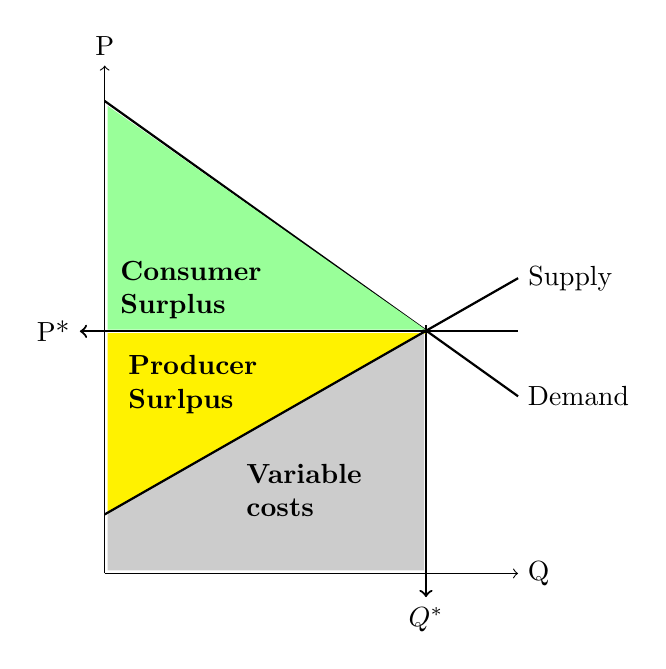
\begin{tikzpicture}[scale=1.5]
%\draw[thick,color=gray,step=.5cm, dashed] (-0.5,-.5) grid (3,3);
\draw[->] (0,0) -- (3.5,0) node[right ] {Q};
\draw[->] (0,0) -- (0,4.3) node [above] {P};
\draw[thick] (0,4) -- (3.5,1.5) ; \node [right]at (3.5, 1.5 ) {Demand}; 

\draw[thick,->] (2.72,2.1) -- (2.72,-.2) node[below] {$Q^*$};
\filldraw [color=green!40]  (0.03,2.07)-- (0.03,3.95)--(2.7,2.07)--cycle;
\filldraw [color=yellow] (0.03,2.03)-- (0.03,.515)--(2.7,2.03)--cycle;
\filldraw [color=gray!40](0.03,.515)--(2.7,2.03)-- (2.7,0.03)--(0.03,0.03)--cycle;
\draw[thick,<-] (-.21,2.05)node[left]{P*}  -- (3.5,2.05) node[above left] {}; 
%\fill[blue, opacity=.25]  (0,4) -- (1.86,2.1) --  (0,2.1) --cycle; 
%\fill[green] (0,.52) -- (1.82,2.1) --  (0,2.1) --cycle; 
\draw[thick] (0,.5) -- (3.5,2.5) node[right] {Supply};
\path (.7,2.4) node [text width=1.7cm](labelRent) {\textbf{Consumer\\ Surplus}};
\path (.7,1.6) node [text width=1.5cm](labelRent) {\textbf{Producer\\ Surlpus}};
\path (1.7,.7) node [text width=1.5cm](labelvarcost){\textbf{Variable\\ costs}};
%\path (1.7,-1) node [black](labePC) {With producible capital};
\end{tikzpicture}     
\caption{The modern concept of producer surplus is graphically and logically equivalent to Ricardian rent.}
\label{fig-producer-surplus}
\end{center}
\end{figure}


\section{Rent in modern economic theory} \label{section-rent-modern-economics}
Neoclassical economics has not abandoned rent theory. It has simply moved it to the side to focus  on %the exchange price and the marginal conditions satisfied in exchange, 
other topics which marginalist techniques explain more satisfactorily. Despite this, the  classical concept of rent  is embedded in a great deal of standard analysis.

The most obvious place that rent persists in modern microeconomic theory is in the concepts of `\gls{consumer surplus}' and `\gls{producer surplus}'  Both of these concepts are illustrated in Figure~\ref{fig-producer-surplus}. They are both variants of rent and are essential in demonstrating the efficiency of markets and the social losses due to \gls{monopoly}, \gls{monopsony}, regulation, and taxes. Consumer surplus is the sum of rents that accrue to the class of consumers (buyers). Producer surplus corresponds precisely to land rent. It is an \gls{inframarginal} quantity, that accrues to the class of landowners. It arises because consumers have differing capacity to produce  utility with the good, just as landowners have lands with different abilities to produce agricultural output.\footnote{See the similarity between the \gls{producer surplus}, illustrated in Figure~\ref{fig-producer-surplus} and in Figure~\ref{fig-rent-ricardo}, illustrated \gls{rent} in the story of the carter.}

Other significant examples of rent in modern microeconomic theory include: 

 % ADD BACK *** Modern economists generally focus  on the exchange price and the marginal conditions satisfied in exchange, which neoclassical economics explains more satisfactorily They appear to have abandoned rents as a central concept, but it  persists in slightly covert forms at the centre  neoclassical economics. 
\begin{enumerate}

\item  %first year students learn that 
The high salaries of sports stars are explained as rents on their scarce talents. %This concept of rent is so central, it is taught to first year Economics students as part of the mainstream curriculum.

\item The ``First Fundamental Theorem of Welfare Economics,'' proven independently by Kenneth Arrow \cite{arrowExtensionBasicTheorems1951} and  Gerald Debreu \cite{debreuCoefficientResourceUtilization1951}  in 1951, is possibly the most significant theorem in the social sciences. It demonstrates that perfectly competitive markets would maximize producer and consumer surplus, quantities that  are variants of rents.

\item The theory of \gls{rent-seeking}  became the subject of durable interest among economists and political scientists after the publication of two influential papers on the topic by Gordon Tullock in 1967 \cite{tullockWelfareCostsTariffs1967}, and Anne Krueger \cite{kruegerPoliticalEconomyRentSeeking1974} in 1974. Rent-seeking occurs when an someone seeks to increase their own wealth without creating any benefits or wealth to the society. Financialization, as we use the term, is a variety of rent-seeking.

\item In resource economics \gls{economic rent}, defined as ``a money payment made for a factor of production that is over and above the minimum payment to keep it in its present use,'' is a central analytical device \cite{Gray1914RentUT}.   
    
\end{enumerate}

As we will discuss in detail in Chapter~\ref{chapter-space}, the classical concept of rent is also at the heart of modern urban theory, although that work does not bring forward the distributional aspects of the classical analysis. The \gls{bid-rent curve}, the value of the bid, or what people will pay to live near the center, became a dominant device in urban theory with William Alonso's 1961 thesis \cite{alonsoTheoryUrbanLand1960} and the work that followed. %, although the idea has deep roots and others were exploring the principle at the same time.  % DEFINE BID-RENT, LINK WITH REST OF THESIS.


 
\section{Summary}
%Neoclassical theory represented a shift in the central apparatus of economic theory that made sense in the context of three broader shifts in the world/environment/context. First, the shift to industrial production, as manufacturing became increasingly central to output, where, unlike with fixed land stock, new companies could enter and compete away profits. 

% MODE OF PRODUCTION
% STATE OF THE WORLD
% METHODOLOGICAL FRONTIER

% ACTUALLY MARKS A SECOND THEORY OF DISTRIBUTION.
% PROFIT COMPETED AWAY, 
 % successful and captured something important

% With the centrality  and the success of the neoclassical approach, with essentially a different underlying model of how the economy distributes surplus value, rent has played less of a central role.
In this chapter, we have examined the historical development  of rent theory and its role in distribution theories as the necessary background for our development of a modern theory of urban rent. We explained how the concept of economic rent arose in an agricultural economy, and who gets the rents in that type of economy. We then gave an account of how rent theory and the classical distribution theory was pushed into the background as neoclassical theorists analysed the industrial market economy that emerged after the industrial revolution using the  modern theory of production. 

We have also sketched the two great theories of \gls{distribution} in economics. The first is based on the classical concept of rent as explained  by David Ricardo \cite{ricardoEssayInfluenceLow1815}, in which owners of land are able to extract a value beyond what they contribute based on their ownership of a scarce resource. The second is the marginalist approach, developed by John Bates Clark and others, in which workers and other factors  in competitive markets receive the \gls{marginal value-product} of their contribution to production. The two theories coexist and even mingle in modern economics, but it is the marginalist approach that dominates economic teaching. 

Both theories developed in response to the social and economic conditions of the periods in which they emerged. Both attempt to explain where the output of society ends up within society. They are, at their heart, stories of who %can or does 
claims what share of production.
The classical theory of rent linked a spatially distributed economy, agriculture, with the class structure of the society of the time. The neoclassical approach does not contradict the classical view of rents, it simply displaces the analysis to the point where a competitive equilibrium prevails, and shifts attention away from the distribution of land rents.  \footnote{Carey and Lachim \cite{careySomethingNothingHow2019} observe,  however,that, ``[t]he persistent and growing profit share across a range of advanced economies and within industries fundamentally challenges the assumption of perfect competition and suggests that growing market power is at the heart of many of the economic challenges in America today.'' } 

Following the eras of agricultural and then industrial dominance,  we are now arguably in a era dominated by a third mode of production centered on  human capital and urban production. %\footnote{When a new dominant mode or age emerges, the old one doesn't go away. Stone work and bronze work still persist, agriculture and industrial production still persist, they are not however the force driving economic and social relations in the way the were when they were dominant as technologies and modes of production\cite{oldworldsdon'tdie}} 
This new mode of production does not yet have a corresponding theory of distribution. This thesis works to fill that gap by re-introducing rent in the classical sense within an urban model which distributes wages and profits as prescribed by  the neoclassical model. In the next chapter we introduce a 20$^{th}$ century urban model that is essentially an application of classical rent theory.


%Rent is important in this new economy---and takes a rising share---contradicting Marshall.

 % \Gls{class} structure, or how different classes participate in production changes over time as modes of production change. When Ricardo was writing, the economy was still largely reflected feudal social relations in that most land ownership originated in feudal military power. %Even the land of the nobility was divided up into smaller parcels run by knights or vassals. Both of these groups traded military support for land in the local manors. As higher ranking people, knights often presided over an entire manor, while vassals presided only over the land needed to support their families.
 % (IE DESCRIBE role of labour land, capital under feudalism and how this was changing in that period.) 
 
% ADD The evolution of the mode of production has continued, with human capital rather than land or industrial capital increasing the source of the social surplus. The concept of rent is specifically relate to surplus and enabled Ricardo to first talk about how is key to distribution within the economy, amongst classes.  Ricardo essentially developed his concept of Rent to explain the dynamics of distribution between classes. 
% The distribution of rents in the urban model affects urban productivity in our model.
%***E FINANCIALIZATION IS ABOUT SURPLUS. CURRENT THINKING ABOUT FINANCIALIZATION HAS NOT BEEN NOT BEEN PUT INTO A FORMAL MODEL. FORMAL MODELS COME FROM COME FROM THE NEO-CLASSICAL TRADITION. 



% The need to be near a market or prodduction center is easily seen by considering a population at the carrying capacity of the land with individuals supporting themselves using purely local resources. There can be no land rent in this case. If a city rises that must be supplied from those still on the land, land close enough to the city will generate land rent. The value of the land is created by proximity to the city.

%  no separate and comprehensive data are provided on the amounts of land rents and subsoil rents charged and earned, because they are not officially regarded as part of value-added, and consequently are not included in the calculation of GDP (except for the value of productive lease contracts)     https://en.wikipedia.org/wiki/Differential_and_absolute_ground_rent#Rent_in_macro-economics    \href{https://en.wikipedia.org/wiki/Differential_and_absolute_ground_rent#Rent_in_macro-economics}{Wikipediat article on differential rent}


%   *****. \subsubsection{MOVE/CUT? Profit vs rent in the story of the carter}
% % PROBABLY LOTS OF EXTRA TO COMMENT OUT HERE
% We have illustrated the story using a carter with a monopoly on transportation services. If instead there were a monopoly landowner, and the transportation industry were competitive, the landowner would pay carters and farmer workers their minimum cost and keep the profit. In this case economists would call the monopoly profits \glspl{rent}. If the carter claims the surplus, we tend to call it \gls{profit}. If the landowner claims it, we tend to call it \gls{rent}. This is simply because the carter has to invest some capital, buy a cart, etc. For rents, you have to subtract the costs used to produce it. You didn't create the land, so the whole of the surplus can be expropriated. With the capitalist surplus, part of the surplus has to be appropriated to keep generating it. % bringinb tack the inheritance of one line of thinking, the common element that was actually prior in the analysis. That's why Marshal called it quasi-rent- because it will be competed away by tghe structure---it's not jsut the source, but the dynamical or transient nature of the surplus that makes it different.
% cities don't die. it's hard to make land rents disapear for varous reasons. When you tghink about converting it \dots it's a spatial rent, that part of the land rent is a spatial rent, the land is diffferentiated spatially as ricardo's extensive margin.. someone else can expropriate a spatial rent other than the landowners
% debate about rban land rents- infinitely divisible  and urban center coudl in pricnicple move.. 
% Yes urban centers are a tiny share of land, and yes in priciple they could be someone else, but in pracitce they can't. it's the people around it, and hte links airports to other centers, that make it the center. yess you can relase by going higher or changing zoning- realaxine potential energy\dots all that realiese is predicated on the fact that there is this spatial structure already.
% Modern work - develoepr is investing a certain amount to make living space.. described in xyz -- cite future work. not appropraiteing surplus
% CLARIFY - THEY ARE NOT RENTS IF THEY CARTER GETS THEM? WHAT DO WE CALL THEM %\footnote{In the modern economy, agricultural land rents may be captured by corporations,  either by owning the land or by controlling the supply chain.}  
 
 % MOVE? Landlord income in this example is thus a locational \gls{land rent} that exists because of the land's proximity to the market.

 
% Marshall's understanding of quasi-rents, or profits, that the surplus does not stay fixed relative to a good's distance from markets, prices come down. Goods get cheaper. If there is a profit, that's an incentive for another business to enter. There's a return to the owner of a factory, but if it's \gls{competitive}, there's free entry, and other businesses can come in and undercut the factory's price. New entrants compete away the profits, driving the price towards the costs of production.


%   ******. The distribution of these surplus incomes are not explained by the later neoclassical theory. 
%In fact they are assumed to be a transitory phenomenon that disappears as a result of free competitive market entry, even though profits and rents remain a substantial part of national income (20--25 percent) \cite{GET_Britannica} %\footnote{Schmitt, Hans Otto, Pen, Jan, Boulding, Kenneth E. and Kleinsorge, Paul Lincoln. ``distribution theory.'' Encyclopedia \cite{GET_Britannica},  \url{https://www.britannica.com/topic/distribution-theory}. Accessed 22 February 2023.} 
% in the world the neoclassical model describes. 

% - describes an environment on the other end of the spectrum without market power- rent describes in a sense a generalization as if the landlord had perfect market pwoer, now the company creates things but has no power.

% As industrial production grew and eventually exceeded agricultural output. 
% {\color{red}
%Adam Smith 
% A monopoly granted either to an individual or to a trading company has the same effect as a secret \dots The monopolists, by keeping the market constantly under-stocked \dots sell their commodities much above the natural price \dots the price of free competition \dots
% The exclusive privilege of corporations, statutes of and apprenticeship, and all those laws which restrain, in particular employments, the competition to a smaller number than might go into them, have the same tendency, though in a less degree. They are a sort of enlarged monopolies, and may frequently \dots in whole classes of employments keep up the market price of particular commodities above the natural price \dots Such enhancements of the market price may last as long as the regulations of police which give occasion to them. wealth of nations
% }


% \subsection{Social context following WWII}
% % \subsubsection{The marginalist approach}


% Following WWII there were rising wages, relatively \dots

% The formalisms also got taken up in part be
%    *****.  Samuelson's successes brilliant and definitive, the most exciting thing to study in the 1950s and early 1960s, exactly the time when the baby boom drove the largest expansion of the university system in history. Scholars coming from the leading economics departments, had studied Samuelson's work, and now had a chance to build out new departments, and frame curriculum that institutionalized Samuelson's division of economics into macro and micro, econometrics, and position the larger older bidet of work outside as heterodox.\footnote{Young scholars seeking good positions, during the Cold War under McCarthyism, might also have had an inclination to downplay the distributional consequences of their work, or it's connection with classical rent theory, a central part of Marx's analysis.} % economs becone this new syntheis.the moment of oppportunity the math.. a new approach. Institutionalizing a set of new
% % worked so well and 
% Also aligned well with the ambitions and the new position of the US as a world power after WWII exhausted the European powers.

% older called political economy 
% It also suited the times.

% % % \subsubsection{It leaves things out}



% If the inframkargian workssre
% pays every on their marginal share

% the workers as a whole are not geting the mar

% no rent, non of the share of the ruplus

% all workers equal and all firms are equal..

% there is more productive land inframarfinaly 
% and there is more closer to the market inframarginally


% what has disappeared in here is that integral of the inframarginal rents.
% It's disappeared from the analysis, and it has really great distributional consequences.


% that worker ends up getting surplus, it's their own surplus, because its the value of their time that is being valued more highly in the market, and they benefit.

% but those who value more highly being closer to the city, are having that surplus extracted as the surplus
% if they own they land get it, as the worker does. 
% if a landowner owns it, as in the feudal system, a landowner gets it. 

% defend a rent based appraoch to urban distribution.







% \subsection{Mathematization}

% A formal relationship between xyx was increasingly important as the field got more formal/mathematical.

% Math had a long history in economics going back to the French engineers school of roads and bridges.



% The \gls{neoclassical} approaches to economic analysis built on the classical framework. They added  mathematical modelling and the use of calculus. Calculus made it much easier to derive formal statements of what came to be called `marginal conditions,' or rules for efficient choice. It also allowed economists to derive clear rules for complex cases that were difficult to state verbally. For example, the utilitarian goal of ``the greatest good for the greatest number'' which %is comprehensible but vague 
% could be translated into a guideline expressed in terms of the sums of individual marginal utilities equalling the marginal social cost for each good. 

% %*E THIS PARAGRAPH SEEMS TO MOVE  FAST %i THINK YOU NEED TO EXPLIAN MARGINAL CONDITIONS IN MORE DETAIL, REALLY MAKE THAT CLEAR THEN BUILD OUT THE UTILITARIAN GOAL AS MORE OF A FLESHED OUT EXAMPLE. IT SEEMS LIKE THE SKELETON OF WHAT YOU NEED TO INTRODUCE THESE CONCEPTS CLEARLY IS HERE BUT NOT ENOUGH. 

%  *****.   \subsubsection{The Cobb-Douglas Production Function}
% The above functions say what the factors of production are that shape output. They don't say what the function is: there's no specification of how the factors relate to output. Developing a more formal theory, in an age before computers where equations and calculus were the cutting edge for formal analysis, required specifying particular functional forms.

% In 1928, mathematician Charles Cobb and Economist Paul Douglas came up with a specific and convenient functional form \cite{cobbTheoryProduction1928}\footnote{The function had apparently previously been used by Knut Wicksell, Philip Wicksteed, and L\'eon Walras.} that captured much of what economists were talking about. The function is just a \gls{generalized arithmetic mean}:
% \[Y=AK^\alpha L^\beta\]
% where $A$ is a constant scale factor, now commonly called \gls{total factor productivity}. This function becomes the workhorse of neoclassical growth theory in the second half  of the 20th century. Our urban model is a direct heir to developments in neoclassical growth theory.
 
% The Cobb Douglas function has several convenient features. One is that the sum of the coefficents tells us the degree of returns to scale. If $\alpha+\beta = 1$, we have \gls{constant returns to scale},

% %Another is that the coefficients of the factors, $\alpha$  and $\beta$ turn out to be the elasticities of output with respect to capital and labour respectively as well as the income share of the factor. These made it relatively easy for economists to combine national data on labour and capital stocks or income with output to test the model.

% The Cobb-Douglas form was developed and almost immediately tested against statistical evidence in the USA by Cobb and Douglas between 1927--1947. It was  their widely circulated empirical work seems to have permanently associated this simple function with Cobb and Douglas for economists.


%I have not followed this track down to give references.

% ALSO Imperfect Competition and \gls{total factor productivity} Growth  AZZEDDINE M. AZZAM, ELENA LOPEZ and RIGOBERTO A. LOPEZ. Journal of Productivity Analysis. Vol. 22, No. 3 (November, 2004), pp. 173-184 (12 pages)

%Sjak Smulders and Theo van de Klundert.Imperfect competition, concentration and growth with firm-specific R & D European Economic Review. Volume 39, Issue 1, January 1995, Pages 139-160
% Duranton, Gilles (1997) Essays on growth: imperfect competition, labour supply and local public goods. PhD thesis, London School of Economics and Political Science.  http://etheses.lse.ac.uk/1471/1/U105715.pdf

%\footnote{Alberto Bucci.  R&D, Imperfect Competition and Growth with Human Capital Accumulation, 2003. Scottish Journal of Political Economy. https://doi.org/10.1111/1467-9485.5004004. This paper studies the long-run consequences of imperfect competition on growth and the sectoral distribution of skills within an R&D-based growth model with human capital accumulation. We find that steady-state growth is driven only by incentives to accumulate skills. In the model imperfect competition has a positive growth effect, while influencing the allocation of human capital to the different economic activities employing this factor input. Contrary to general wisdom, the share of resources invested in R&D turns out not to be monotonically increasing in the product market power and its correlation with the equilibrium output growth rate is not unambiguous.}

%NOTE URBAN COMPETITION PROVIDES INCENTIVES TO UPGRADE SKILLS!!!


% Both the Solow (1956) growth model and its Ramsey-Cass-Koopmans counterpart featuring an endogenous saving rate (Ramsey, 1928; Cass, 1965; Koopmans, 1965) but treat technical change as purely exogenous. In fact, under the assumption of perfectly competitive goods and factors markets as well as marginal productivity pricing of capital and labour, neoclassical growth requires technical change to be generated outside the model because there are no resources left to innovate if both factors of production. 

% 
% assuming that technical progress is labour augmenting (Uzawa, 1961), we can rewrite the production function as $F(K, AL$), where $AL$ is a measure of labour in efficiency units, or effective workers. Let k = K/(AL). Then, output per effective worker is y =Y/(AL)=f (k). Population grows at the constant rate n > 0 and, as we will assume throughout the whole paper, capital does not depreciate. The steady state of the Solow model solves

% $\frac{f(k_{ss}}{k_{ss}} = \frac{n+g_A}{s}kss s$

% Journal of Economic Surveys (2017) Vol. 31, No. 5, pp. 1272--1303 \c ECONOMIC THEORIES 1275



% HOUSING RENT IN THE NATIONAL ACCOUNTS
%   Owner-occupied housing is included in Personal Consumption Expenditure because the National Income and Producgt Accounts (NIPAs) treat the owner-occupant as if it were a rental business, or in other words, a landlord renting to him or herself. That is, BEA imputes a value for the services of owner-occupied housing (space rent) based on the rents charged for similar tenant-occupied housing, and this value is included in GDP as part of personal consumption expenditures. This imputation is necessary in order for GDP to be invariant when housing units shift between tenant occupancy and owner occupancy.

%Ricardo  clearly understood and used the concept of diminishing marginal product. This shows in his use of the terms ``extensive margin'' and ``intensive margin'' to explain the income of the landowner. He focussed on the difference between the cost of production on a unit of land and the revenue generated. The landlord would rent out all the land which generated at least enough to pay all the costs. Anything in excess of the costs could be charged as land rent to a tenant farmer.

%Clearly in his model there are two basic productive factors, land and labour. The landlord  receives the surplus generated by the land and the rest of the value of production goes to labour. 


% \subsection{Marginalist dis tribution}
% MARGINALIST DISTRIBUTION
% we've been paying some people less than the market wage so our profits our higher. this is what it would be if we paid everybody

% FOOTNOTE - RELATIONSHIP with marginalist distribution story ******** TODO Does the marginalist approach assume they are not exploited? Is it an experiment in examining the case where production is non-exploitative? 
% In a sense if labour gets the marginal value of their product, are they exploited. It's a matter of interpretation.  -It has an attraction 
%Clark tried to make an ethic of this. if everyone is being paid the marginal product of their labour. We know that's an efficient outcome. If it's efficient, is it also fair
%Is it possible someone's taking out an extra large fair. Yes. Not fair for simple classical reason that labour has been exploited in the past and that the current owner ship is a result of exploitation. The ownership of land introduces a kind of exploitation-- clearly exploitation if you claim that. 
%Lot's of marxists didn't like Henry George making it a locational question, they wanted to keep it located in the factory.
% You could - well what value did they create---in line with those other-- could interpret.. 
%What is the average value, because every worker is not just marginal, they're also average/identical. What is the value created by the whole of the workforce. Should they be paid the marginal value or the average value of their work.
%
%The avg value---declining.. 
%The demand for labour is declining--  
%Every infra marginal worker has been paid less than the avg contribution 
%Every infra marginal workers should - 
%every marginal worker should get the average wage.. that's fair.

%Get to the margin - that's what you pay.. that's what the next worker is worth to the firm. .. 5th' worker is paid more than the 10th. should it be averaged out and paid to all workers? paid to worker, or should the difference between top and the marginal goes to the firm---that's profit.. pay everyone the marginal value and keep the rest as profit.. 
%Effective labour has a higher marginal product.. - even higher - higher for the firm.. - but they don't have to pay the workers that \dots firms only have to pay enough to get their marginal individual cost down to the wage. The problem there is if they're making more profit they want to expand the workforce, but that wage only supports a certain size of city---they've got off raise the wage a bit.. so they face an upward sloping supply curve for labour=-- that's why you know there's an equilibrium.. declining product and upward sloping supply so they cross.

%(all the profit you earn on the way could be redistributed)



% \section{Human capacity - A new theory of urban rent for an age of human capacity}
% % \section{New methods- Agent based models}
% They depended on equations and calculus and could say only a few things formally.
% They had to talk in averages, about average distribution, and lost what that meant for the individual.

% We now have tools that let us richly model the kinds of complex ideas 

% We are at a time with a new mode of production centered on human capacity, intellectual property, and financial innovation. %

% We have seen a massive return of inequality and consolidation of wealth which should not be seen according to to the neoclassical theory % GET REFERENCES

% We have yet to make a new theory of distribution for the new world.
% % (selling debt of various kinds- literal promises against the futuer which will one day be used up in our speculative frenzy.)


% all these 3 things have shifted - a new dominant mode of production, rising inequality not explained by the prior mode, and mathematics of agents that lets us talk about big rich ideas again.

% % abundance super choice..
% % MISSES THE STORY INEQUALITY SHOULDN'T HAPPEN - CRYSTIA FREELAND..
% % suited to the economic reality---rising equality and wages following WWII. Massive inequality now..
% we're in a new reality, but doesn't have a new economic theory for it. 

% Late in the 20$^{th}$ century, the focus shifted again, to the economics of  knowledge, human capital, and how cities generate wealth, a change that plays a part in  our theory of urban rents in Chapter~\ref{chapter-growth}. 
 
% The changes have tracked changing social relations. The influence of landowners declined and the power of industrial capitalists increased throughout the 19$^{th}$ century. More recently the owners of industrial capital have been eclipsed, to some extent, by financial capital and by the owners or creators of certain information technologies.
